\documentclass[11pt]{beamer}
\usepackage{verbatim}
\usepackage{amsmath}
\usepackage{amsthm}
\usepackage{graphics}
\usepackage{color}
\usepackage{stmaryrd}\usefonttheme[onlymath]{serif}

\title{On Multiphase-Linear Ranking Functions}
\date{\today}
\author{Xie Li}

\begin{document}
\maketitle


\begin{frame}\frametitle{Single Path Linear Constraint Loop}
\begin{example}
\begin{center}

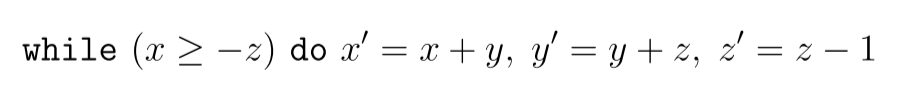
\includegraphics[scale = 0.4]{loopExample.png}

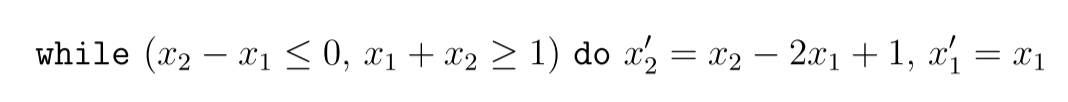
\includegraphics[scale = 0.4]{loopExample1.png}
\end{center}

\end{example}

\begin{definition}[SLC]
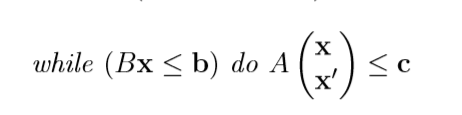
\includegraphics[scale = 0.4]{1.PNG}


\end{definition}
\begin{center}
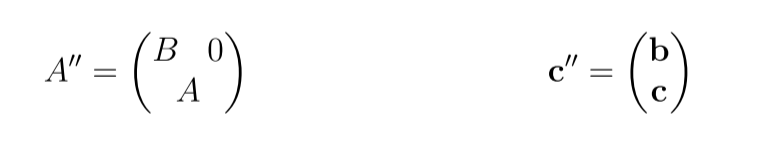
\includegraphics[scale = 0.35]{2.PNG}

$A''\textbf{x}'' \le \textbf{c}''$
\end{center}


\end{frame}

\begin{frame}\frametitle{Ranking Functions}

\begin{definition}[Linear Ranking Function(LRF)]

$f(x_1, \ldots, x_n) = a_1x_1 + \ldots a_nx_n + a_0$, such that

\begin{itemize}
\item $f(\textbf{x}) \ge 0$ for any $\textbf{x}$ satisfies the loop constraints.

\item $f(\textbf{x}) - f(\textbf{x}') \ge 1$ for any transition from $\textbf{x}$ to $\textbf{x}'$.



\end{itemize}
\end{definition}

\begin{example}
\[\texttt{while }( x - 1 > 0) \texttt{do } x' = x - 5\]

Its LRF: $f(x) = x - 1$
\end{example}

We can define a binary relation $\textbf{x} \succeq \textbf{x}'$ iff  $f(\textbf{x}) - f(\textbf{x}') \ge 1$ and $f(\textbf{x}) \ge 0$

\end{frame}

\begin{frame}\frametitle{Nested r.f.}

\begin{definition}[Nested Ranking Function]

A tuple $\langle f_1, \ldots, f_d\rangle$ is a nested ranking function for $T$ if the following requirements are satisfied for all $\textbf{x}''\in T$
\begin{center}
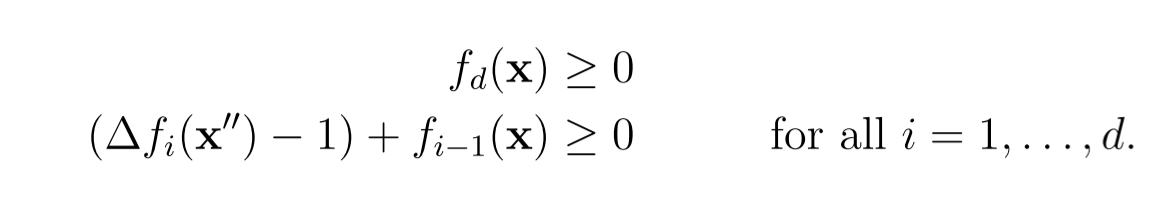
\includegraphics[scale = 0.3]{6.PNG}

\end{center}

Let $f_0 = 0$.
\end{definition}


\end{frame}
\begin{frame}\frametitle{Example: Multiphase Ranking Function}
\[\texttt{while }( x > -z) \texttt{do } x' = x + y, y' = y + z, z = z - 1\]

Attempt to use a ranking function that has several phases: 
$\langle z + 1, y + 1, x\rangle$
\begin{center}
\begin{tabular}{|c|c|c|c|c|c|}
\hline 
$x$&$y$&$z$&$z+1$&$y+1$&$x$\\
\hline
$1$&$1$&$1$&\textbf{2}&$2$&$1$\\
$2$&$2$&$0$&\textbf{1}&$3$&$2$\\
$4$&$2$&$-1$&\textbf{0}&$3$&$4$\\
\hline
$6$&$1$&$-2$&$-1$&\textbf{2}&$6$\\
$7$&$-1$&$-3$&$-2$&\textbf{0}&$7$\\
\hline
$6$&$-4$&$-4$&$-3$&$-3$&\textbf{6}\\
$2$&$-8$&$-5$&$-4$&$-7$&\textbf{2}\\
\hline
$-6$&$-13$&$-6$&$-5$&$-12$&$-6$\\
\hline
\end{tabular}
\end{center}
\end{frame}


\begin{frame}{Multiphase Ranking Function}
\begin{definition}
Given a set of transitions $T\subseteq \mathbb{Q}^{2n}$, we say $\langle f_1, \ldots, f_d\rangle$ is a multiphase ranking function for $T$ if for every $\textbf{x}'' \in T$, there is an index $i\in [1, d]$, s.t.

\begin{center}
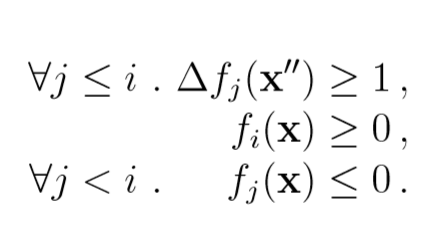
\includegraphics[scale = 0.3]{3.PNG}
\end{center}
We say that $\textbf{x}''$ is ranked by $f_i$(for the minimal).
\end{definition}


\end{frame}


\begin{frame}\frametitle{Example Revisit}
\[\texttt{while }( x > -z) \texttt{do } x' = x + y, y' = y + z, z = z - 1\]

\begin{center}
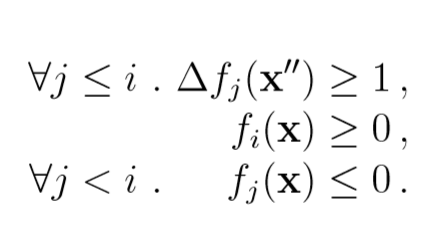
\includegraphics[scale = 0.2]{3.PNG}

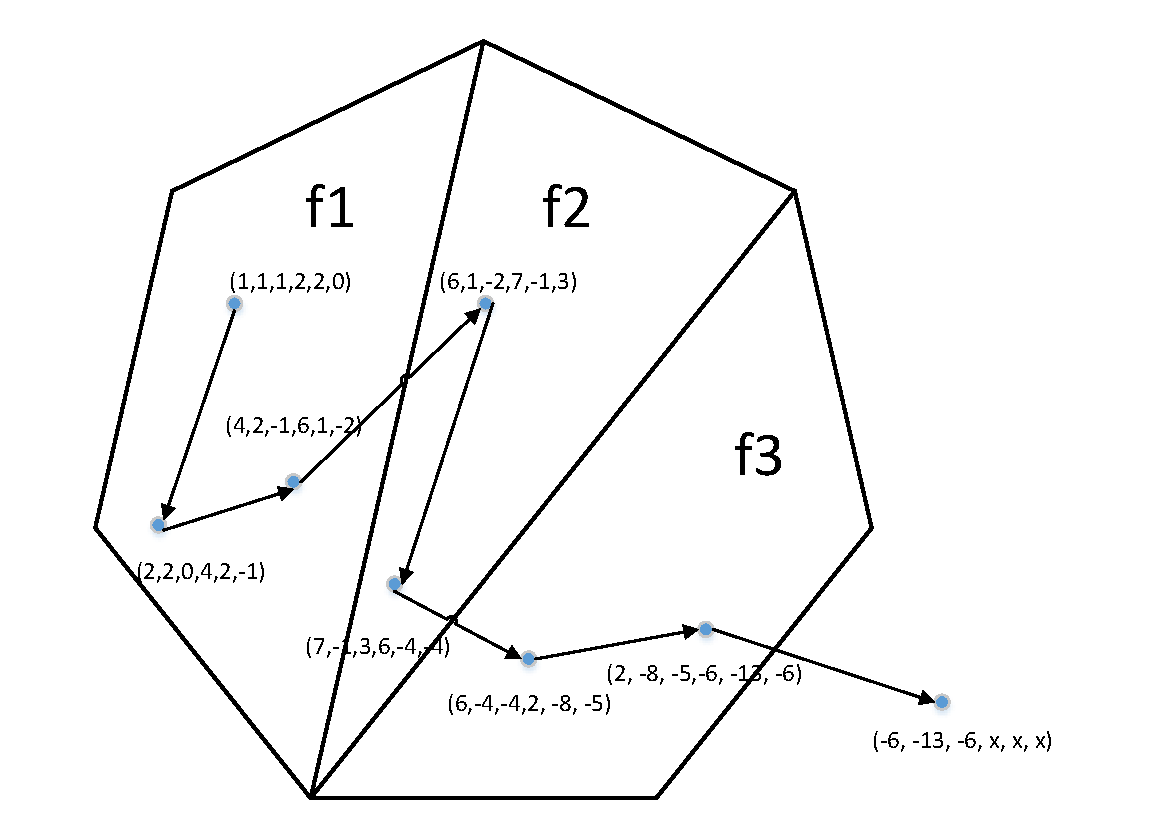
\includegraphics[scale = 0.4]{3.pdf}
\end{center}
\end{frame}




\begin{frame}\frametitle{Motzkin's Transposition Theorem}
\begin{theorem}[Motzkin's Transposition Theorem]
For $A\in \mathbb{K}^{m\times n}, C\in \mathbb{K}^{l\times n}, b\in \mathbb{K}^m, $ and $d\in \mathbb{K}^l$. The formulae below are equivalent.
\begin{itemize}
\item $\forall x \in \mathbb{K}^n. \neg (Ax\le b \wedge Cx < d)$

\item $\exists \lambda \in \mathbb{K}^m. \exists \mu \in \mathbb{K}^l.$

$\lambda \ge 0 \wedge \mu \ge 0$

$\wedge \lambda^{T}A + \mu^TC = 0 \wedge \lambda^{T}b + \mu^Td \le 0 $

$\wedge (\lambda^Tb < 0 \vee \mu \ne 0)$

\end{itemize}
\end{theorem}


Intuition of Motzkin's transposition theorem:...
\end{frame}


\begin{frame}
\begin{lemma}[0]
Given an non-empty polyhedron $\mathcal{P}$ and linear functions $f_1, \ldots , f_k$ such that 

\begin{enumerate}
\item $\textbf{x}\in \mathcal{P}\rightarrow f_1(  \textbf{x}) > 0 \vee \ldots \vee f_{k-1}(\textbf{x}) > 0 \vee f_{k}(\textbf{x}) \ge 0$

\item $\textbf{x} \in \mathcal{P} \not\rightarrow f_1(\textbf{x}) > 0 \vee \ldots f_{k-1}(\textbf{x}) > 0$

\end{enumerate}
There exists a non-negative constants $\mu_1, \ldots, \mu_{k-1}$ such that 

\[\textbf{x}\in \mathcal{P} \rightarrow \mu_1f_1(\textbf{x}) + \mu_{k-1}f_{k-1}(\textbf{x}) + f_k(\textbf{x}) \ge 0\]
\end{lemma}


\end{frame}


\begin{frame}\frametitle{M$\Phi$RF to Nested r.f.}
\begin{theorem}[1]
If $\mathcal{Q}$ has a M$\Phi$RF of depth $d$, then it has a nested ranking function of depth at most $d$.


\end{theorem}

\begin{proof}
By induction on the depth $d$.
\begin{itemize}
\item $d = 1$: M$\Phi$RF and nested r.f. are both LRF.
\item $d > 1$: $d = 2$ e.g.
$\langle f_1, f_2\rangle$. When index $i = 1$, we do not impose bound on $f_2(\textbf{x})$. However, a bound is needed for $f_2'(\textbf{x}s)$ in nested r.f. $\langle f_1', f_2'\rangle$.

To solve the problem that $f_2(\textbf{x})$ might goes under $0$, when $\textbf{x}''$ is ranked by $f_1$. Consider  $\mathcal{Q}' = \mathcal{Q}\cap \{\textbf{x}''\in \mathbb{Q}^{2n}\mid f_1(\textbf{x}'') \le 0\}$


\end{itemize}


\end{proof}

\end{frame}

\begin{frame}\frametitle{M$\Phi$RF to Nested r.f.}
\begin{lemma}[1]
Let $\tau = \langle f_1, \ldots, f_d \rangle$ be an irredundant M$\Phi$RF for $\mathcal{Q}$, such that $\langle f_2, \ldots, f_d\rangle$ is a nested ranking function for $\mathcal{Q}' = \mathcal{Q}\cap \{\textbf{x}''\in \mathbb{Q}^{2n}\mid f_1(\textbf{x}) \le 0\}$. Then there is a nested ranking function of depth $d$ for $\mathcal{Q}$.

\end{lemma}
Prove by construction: construct a nested r.f. $\langle f_1', \ldots, f_d'\rangle$
\begin{center}
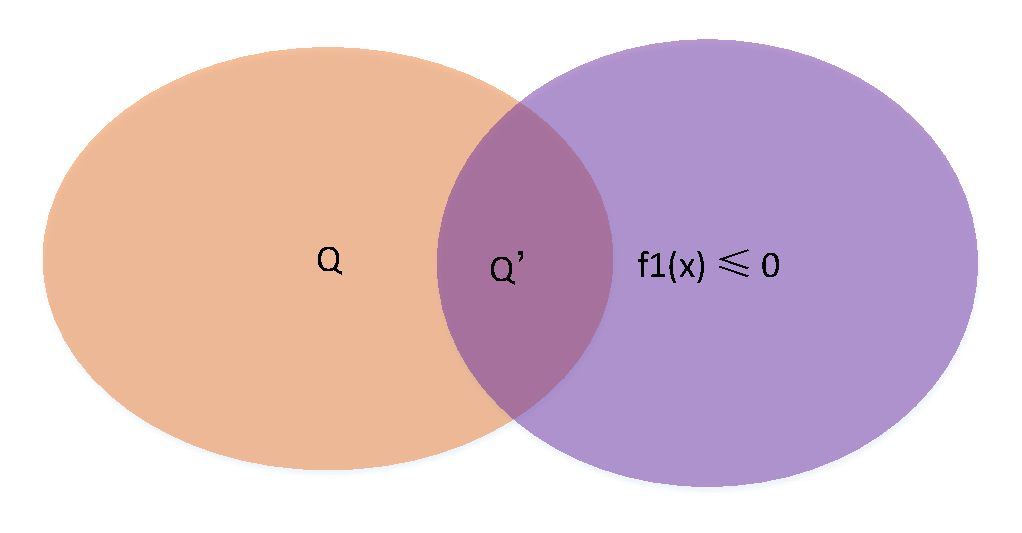
\includegraphics[scale = 0.3]{1.pdf}
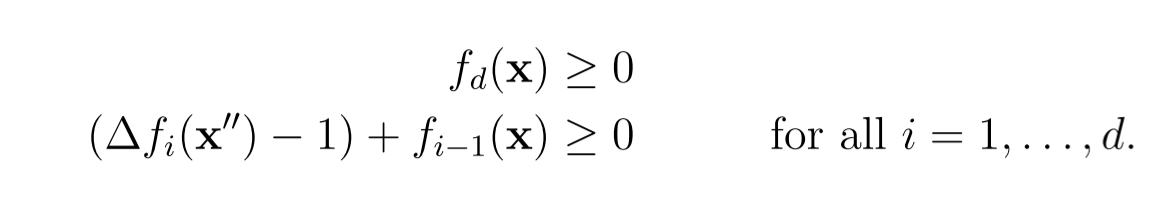
\includegraphics[scale = 0.2]{6.PNG}


\end{center}
If $f_d$ is non-negative on $\mathcal{Q}$, then $f_d' = f_d$.
Otherwise, $\textbf{x}'' \in \mathcal{Q} \rightarrow f_d(\textbf{x}) \ge 0 \vee f_1(\textbf{x}) > 0$


\end{frame}


\begin{frame}\frametitle{M$\Phi$RF to Nested r.f.}
\begin{center}
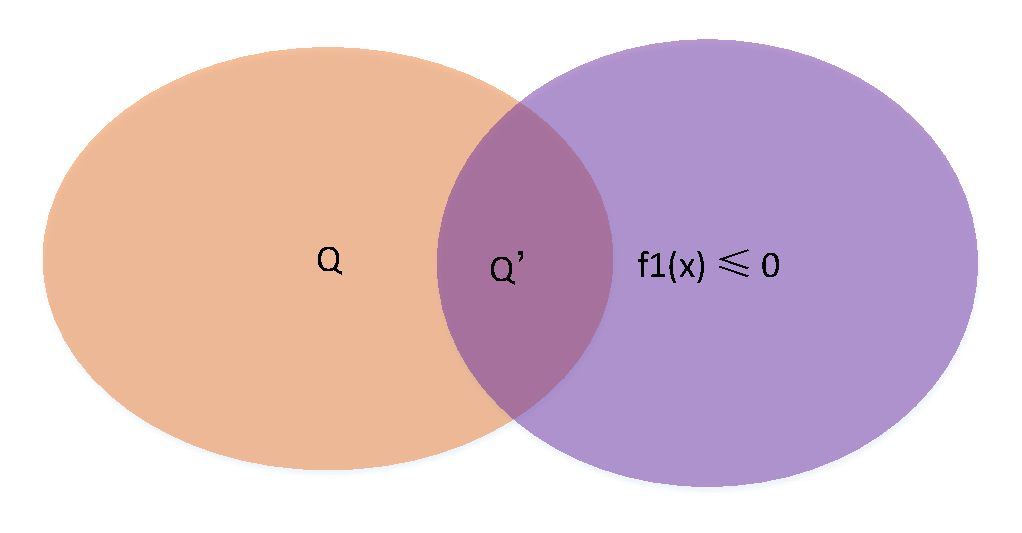
\includegraphics[scale = 0.3]{1.pdf}
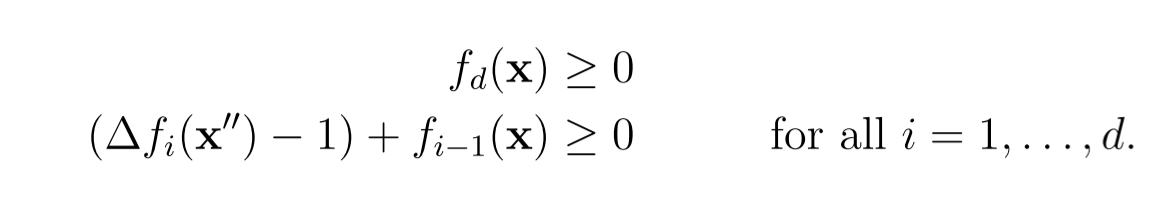
\includegraphics[scale = 0.2]{6.PNG}
\end{center}

Assume $f_{n}'(\textbf{x})= f_{n}(\textbf{x}) + \mu_{n}f_1(\textbf{x})$ and $f_d', \ldots, f_{i}'$ has already been computed.
\[\textbf{x}''\in \mathcal{Q}' \rightarrow (\Delta f_i(\textbf{x}'') - 1) + f_{i-1}(\textbf{x}) \ge 0\]
\[\textbf{x}''\in \mathcal{Q}' \rightarrow (\Delta f_i'(\textbf{x}'') - 1) + f_{i-1}(\textbf{x}) \ge 0\]
If above inequation also holds for $\mathcal{Q}$, then $f_{i-1}' = f_{i-1}$, Otherwise
\[\textbf{x}''\in \mathcal{Q} \rightarrow (\Delta f_i'(\textbf{x}'') - 1) + f_{i-1}(\textbf{x}) \ge 0 \vee f_1(\textbf{x}) \ge 0\]


\end{frame}

\begin{frame}\frametitle{BM$\Phi$RF($\mathbb{Q})\in$\texttt{PTIME}}
\begin{theorem}[2]
BM$\Phi$RF($\mathbb{Q}$)$\in$\texttt{PTIME}.



\end{theorem}

\begin{proof}


\end{proof}
\end{frame}


\begin{frame}\frametitle{LLRF}

Intuition: remind binary relation $\textbf{x} \succeq \textbf{x}'$ iff  $f(\textbf{x}) - f(\textbf{x}') \ge 1$ and $f(\textbf{x}) \ge 0$.

Generalize it into several phases using lexicographical order of ranking functions.

$\langle f_1, f_2, \ldots, f_d\rangle$

$(2,3,1,3) \ge (2,1,5,4)$

\begin{definition}[LLRF]
Given a set of transitions $T$ we say that 
$\langle f_1, f_2, \ldots, f_d\rangle$ is a LLRF (of depth $d$) for $T$ if for every $\textbf{x}''\in T$ there is an index $i$ such that 
\begin{center}
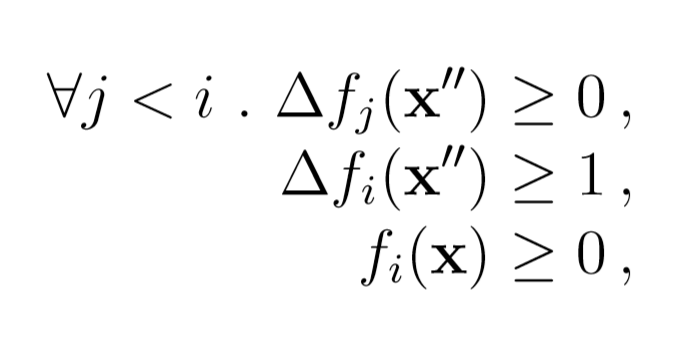
\includegraphics[scale = 0.26]{4.PNG}

\end{center}
A LLRF is weak if..
\end{definition}

\end{frame}

\begin{frame}\frametitle{Weak LLRF to M$\Phi$RF}

\begin{theorem}[3]
If $\mathcal{Q}$ has a weak LLRF of depth $d$, it has a  M$\Phi$RF of depth $d$.


\end{theorem}

\begin{proof}
Prove by induction.

\begin{itemize}

\item $d = 1$: 
For LLRF: $\Delta f_1(\textbf{x}'') > 0$, $f_1(\textbf{x}) \ge 0$ is a LRF due to the loop is linear.

For M$\Phi$RF: is a LRF.

\item $d > 1$: Observe that for a given LLRF $\langle f_1, f_2, \ldots, f_d\rangle $, after removing $f_k$, $\langle f_1, \ldots, f_{k-1}, f_{k+1}, \ldots, f_d\rangle$ is also a LLRF.

If we apply IH here, we get a M$\Phi$RF of depth $d-1$.

\end{itemize}


\end{proof}


\end{frame}


\begin{frame}\frametitle{Weak LLRF to M$\Phi$RF}
Now we want some techniques to use a M$\Phi$RF of depth $d - 1$ and $f_k$ we removed to prove there is a M$\Phi$RF of depth $d$ on $\mathcal{Q}$. 
\begin{lemma}[2]
Let $f$ be a non-negative linear function over $\mathcal{Q}$. If $\mathcal{Q}' = \mathcal{Q}\cap \{\textbf{x} '' \mid \Delta f(\textbf{x} '') \le 0\}$ has a M$\Phi$RF of depth $d$, then $\mathcal{Q}$ has a M$\Phi$RF of depth at most $d + 1$.
\end{lemma}
\begin{proof}
Prove by construction: if the known M$\Phi$RF is $\langle g_1, \ldots, g_d \rangle$ and the funtion non-negative function is $f$, we wish to construct a  M$\Phi$RF $\langle g_1', \ldots, g_n', f\rangle$ of depth $d + 1$
\[\textbf{x}''\in \mathcal{Q} \rightarrow \Delta f(\textbf{x}'') > 0 \vee \Delta g_1(\textbf{x}'') \ge 1\]

Then update $g_2$ to $g_2'$ when $g'_1(\textbf{x}) \le -1$, an so on...

\end{proof}

\end{frame}

\begin{frame}\frametitle{Weak LLRF to M$\Phi$RF}
Remind the $f_k$ we removed in the theorem, together with Lemma(2), we wish to construct a non-negative linear function $g$ over $\mathcal{Q}$ and $g$ decrease on (at least) the same transitions of $f_k$.
\begin{lemma}[3]
Let $\langle f_1, \ldots, f_d\rangle$ be a weak LLRF for $\mathcal{Q}$. There is a linear function $g$ that is positive over $\mathcal{Q}$, and decreasing on (at least) the same transitions of $f_i$, for some $i\in [1,d]$.

\end{lemma}

\begin{proof}
Use Lemma(0) to find the $i$.
\end{proof}

\end{frame}
\begin{frame}\frametitle{M$\Phi$RF and LLRFs over the Integers}
\begin{example}
\[\texttt{while } (x_2 - x_1 \le 0, x_1 + x_2 \ge 1, x_3 \ge 0) 
\]
\[\texttt{do }x_2 ' = x_2 - 2x_1 + 1; x_3 ' = x_3 + 10x_2 + 9\]
\end{example}
Intepreted over integer: the loop has the M$\Phi$RF $\langle 10x_2, x_3\rangle$

Intepreted over rationals: the loop does not terminate: $(\frac{1}{2}, \frac{1}{2}, 0)$


\end{frame}

\begin{frame}\frametitle{M$\Phi$RF and LLRFs over the Integers}

\begin{itemize}
\item Integer case for LRF: completeness for the integer version was achieved by reducing the problem to the rational case. Intuitionly, since $\mathcal{Q}_I$ is the convex combinition of points in $I(\mathcal{Q})$.

\item Theorems above does not apply to the integer versions, but in the following we will prove that the reduction from integer case to rational also works for LLRF and M$\Phi$RF.
\end{itemize}


\end{frame}


\begin{frame}\frametitle{Weak LLRF: Integer to Rational}
\begin{theorem}[4]

Let $\langle f_1, \ldots, f_d\rangle$ be a weak LLRF for $I(\mathcal{Q})$. Then there are constants $c_1, \ldots, c_d$ such that $\langle f_1 + c_1, \ldots, f_d + c_d\rangle$ is a weak LLRF for $\mathcal{Q}_I$(over the rationals).

\end{theorem}


\begin{proof}
prove by induction:

\begin{itemize}
\item $d = 1$, LRF.
\item $d > 1$, define 
\[\mathcal{Q}' = \mathcal{Q}_I\cap \{\textbf{x}''\mid f_1(\textbf{x}) \le -1\}\]
\[\mathcal{Q}'' = \mathcal{Q}_I \cap \{\textbf{x}''\mid \Delta f_1(\textbf{x}'') = 0\}\]

by IH, the theorem holds on $\mathcal{Q}_I'$ and $\mathcal{Q}_I''$ for weak LLRF of depth $d - 1$. say,
\[\langle f_2 + c_2', \ldots, f_d + c_d'\rangle, \langle f_2 + c_2'', \ldots, f_d + c_d''\rangle\]
\end{itemize}

\end{proof}
\end{frame}


\begin{frame}\frametitle{Proof Continue}


\[\mathcal{Q}' = \mathcal{Q}_I\cap \{\textbf{x}''\mid f_1(\textbf{x}) \le -1\}\]
\[\mathcal{Q}'' = \mathcal{Q}_I \cap \{\textbf{x}''\mid \Delta f_1(\textbf{x}'') = 0\}\]
Then we wish to have a lower bound on $f_1(\textbf{x})$.

\[\langle f_1 + c_1, f_2 + \max(c_2', c_2''), \ldots, f_d + \max(c_d', c_d'')\rangle\]

This implies the above formula is a weak LLRF on $\mathcal{Q}_I$. i.e. given a $\textbf{x}''\in \mathcal{Q}_I$, either..., or...

Problem: how to prove the existence of the lower bound?

\end{frame}


\begin{frame}\frametitle{Prove the Lower Bound}
$\mathcal{Q}_I', \mathcal{Q}_I''$. Let $f_i(\textbf{x}) = \vec{a}_i\textbf{x} - b_i$.
\begin{itemize}
\item If $\mathcal{Q}_I'$ is empty, then by the definition of $\mathcal{Q}'$ $f_1$ is lower bounded.

\item Otherwise, prove the lower bound on $\mathcal{Q}_I \setminus \mathcal{Q}_I'$
\end{itemize}


\end{frame}



\begin{frame}

\end{frame}
\end{document}